
\usepackage{tikz}
\usetikzlibrary{arrows.meta, positioning, calc, fit, backgrounds, shadows, shapes.geometric, decorations.pathreplacing}
% --- Colors ---
\definecolor{icmlblue}{HTML}{2E4057}
\definecolor{icmlred}{HTML}{D1495B}
\definecolor{icmlgreen}{HTML}{048A81}
\definecolor{icmlbg}{HTML}{F4F7F6}



% --- Helper for Math Text ---
\newcommand{\mathtext}[1]{{\footnotesize #1}}

% --- Mini Plots (scaled down to fit narrower boxes) ---
\newcommand{\MiniPlotGumbel}{%
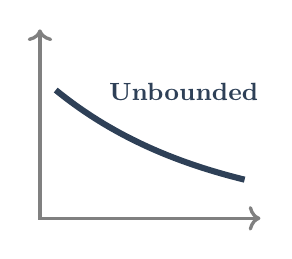
\begin{tikzpicture}[x=2.0cm, y=2.0cm]
  % Axes
  \draw[<->, black!50, line width=1.2pt] (0,1.2) -- (0,0) -- (1.4,0);
  % Curve
  \draw[icmlblue, line width=2.2pt] plot[domain=0.1:1.3, samples=50] (\x, {0.9*exp(-\x)});
  % Label
  \node[font=\bfseries\small, anchor=west, inner sep=2pt, icmlblue] at (0.4,0.8) {Unbounded};
\end{tikzpicture}%
}

\newcommand{\MiniPlotWeibull}{%
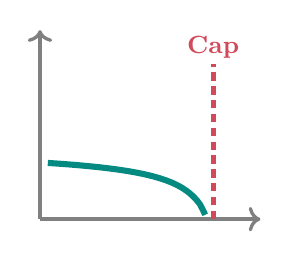
\begin{tikzpicture}[x=2.0cm, y=2.0cm]
  % Axes
  \draw[->, black!50, line width=1.2pt] (0,0) -- (0,1.2);
  \draw[->, black!50, line width=1.2pt] (0,0) -- (1.4,0);
  % Cap Line
  \draw[densely dashed, icmlred, line width=1.8pt] (1.1, 0) -- (1.1, 1.2);
  % Curve
  \draw[icmlgreen, line width=2.2pt] plot[domain=0:1.0, samples=60] (0.05 + \x, {0.5-0.15*pow(1.1-\x, -0.5)});
  % Label kept inside plot to keep bounding box stable
  \node[font=\bfseries\small, anchor=north, inner sep=2pt, icmlred, fill=white] at (1.1,1.2) {Cap};
\end{tikzpicture}%
}




\newcommand{\plotconceptual}{
    \begin{figure*}[t]
    \centering
    \resizebox{\textwidth}{!}{%
    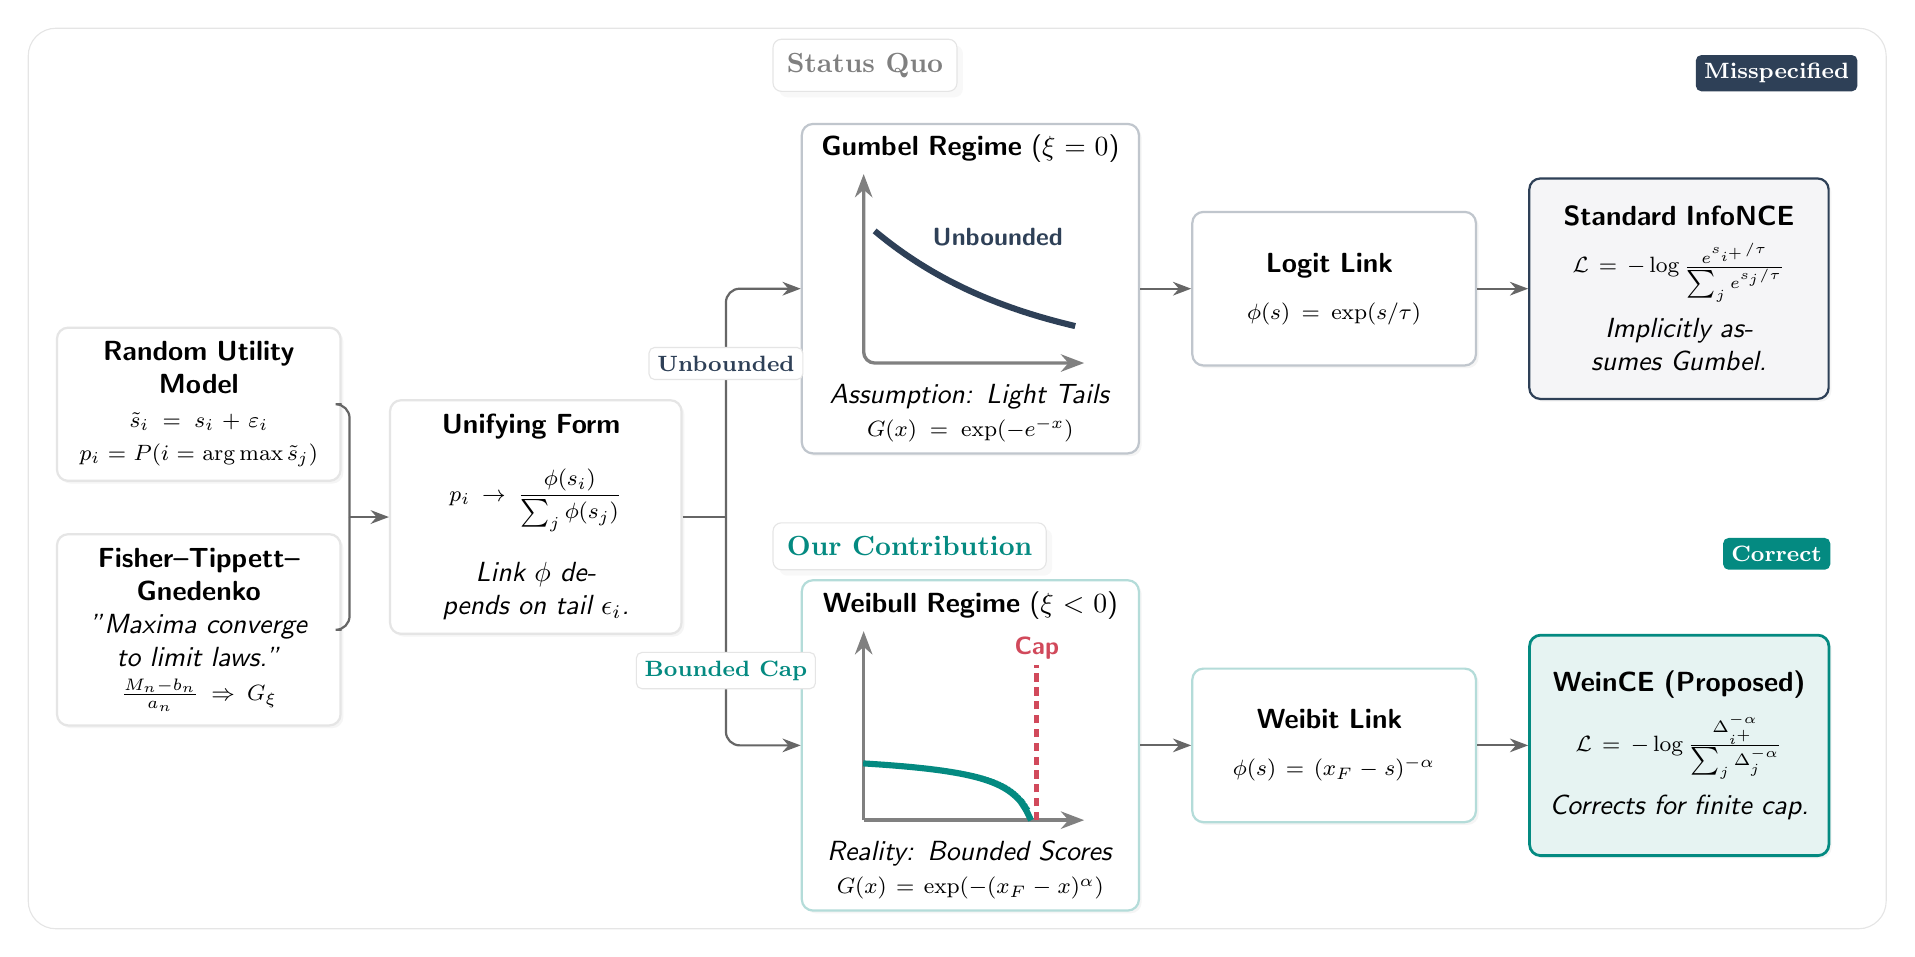
\begin{tikzpicture}[
      node distance=0.7cm and 0.9cm,
      font=\sffamily,
      >=Stealth,
      % --- Base block style ---
      block/.style={
        draw=black!10,
        fill=white,
        rounded corners=4pt,
        line width=0.8pt,
        drop shadow={opacity=0.08, shadow xshift=1pt, shadow yshift=-1pt},
        align=center,
        inner sep=5pt,
        % Bump font up one notch for readability.
        font=\normalsize\sffamily
      },
      % --- Column-specific sizes ---
      smallbox/.style={
        block,
        text width=3.25cm,
        minimum height=1.75cm
      },
      unifybox/.style={
        block,
        text width=3.35cm,
        minimum height=1.55cm
      },
      regimebox/.style={
        block,
        text width=4cm,
        inner sep=4pt
      },
      midbox/.style={
        block,
        text width=3.25cm,
        minimum height=1.95cm
      },
      lossbox/.style={
        block,
        text width=3.45cm,
        minimum height=2.8cm
      },
      arrow/.style={->, thick, draw=black!60, rounded corners=5pt},
      stem/.style ={thick, draw=black!60, rounded corners=5pt},
      branchlabel/.style={
        font=\footnotesize\bfseries\scshape,
        text=black!60,
        fill=white,
        inner sep=3pt,
        rounded corners=2pt,
        draw=black!10
      },
      grouptitle/.style={
        font=\bfseries\normalsize,
        fill=white,
        draw=black!10,
        rounded corners=3pt,
        inner sep=5pt,
        drop shadow={opacity=0.05}
      },
      labeltag/.style={
        font=\footnotesize\bfseries\scshape,
        text=white,
        rounded corners=2pt,
        inner sep=3pt
      }
    ]
    
    % =========================================================
    % Column 1: RUB stacked above FTG (same column)
    % =========================================================
    \node[smallbox] (rum) {
      \textbf{Random Utility\\  Model}\\
      \mathtext{$\tilde{s}_i = s_i + \varepsilon_i$}\\
      \mathtext{$p_i = \mathbb{P}(i=\arg\max \tilde{s}_j)$}
    };
    
    \node[smallbox, below=0.65cm of rum] (ftg) {
      \textbf{Fisher--Tippett--Gnedenko}\\
      \textit{"Maxima converge to limit laws."}\\
      \mathtext{$\frac{M_n-b_n}{a_n}\Rightarrow G_{\xi}$}
    };
    
    % Place UNP in the second column, vertically centered w.r.t. RUB/FTG.
    \coordinate (colonecenter) at ($(rum.center)!0.5!(ftg.center)$);
    % (Use an intermediate coordinate to keep TikZ math robust.)
    \coordinate (unifyx) at ($(rum.east)+(0.6cm,0)$);
    \coordinate (unifypos) at (unifyx |- colonecenter);
    
    % =========================================================
    % Column 2: UNP
    % =========================================================
    \node[unifybox, anchor=west] (unify) at (unifypos) {
      \textbf{Unifying  Form}
      \vspace{10pt}\\
      \mathtext{$\displaystyle p_i \rightarrow \frac{\phi(s_i)}{\sum_j \phi(s_j)}$}\\
      \vspace{10pt}
      \textit{Link $\phi$ depends on tail $\epsilon_i$.}
    };
    
    % =========================================================
    % Column 3: Regimes (two rows)
    % =========================================================
    \node[regimebox, right=1.5cm of unify, yshift=2.9cm, draw=icmlblue!30] (gumbel) {
      \textbf{Gumbel Regime} ($\xi=0$)\\[0.25em]
      \MiniPlotGumbel\\[-0.05em]
      \textit{Assumption: Light Tails}\\
      \mathtext{$G(x)=\exp(-e^{-x})$}
    };
    
    \node[regimebox, right=1.5cm of unify, yshift=-2.9cm, draw=icmlgreen!30] (weibull) {
      \textbf{Weibull Regime} ($\xi<0$)\\[0.25em]
      \MiniPlotWeibull\\[-0.05em]
      \textit{Reality: Bounded Scores}\\
      \mathtext{$G(x)=\exp(-(x_F-x)^{\alpha})$}
    };
    
    % =========================================================
    % Column 4: Links (two rows)
    % =========================================================
    \node[midbox, right=0.65cm of gumbel, draw=icmlblue!30] (logit) {
      \textbf{Logit Link}
      \vspace{5pt}\\
      \mathtext{$\phi(s)=\exp(s/\tau)$}
    };
    
    \node[midbox, right=0.65cm of weibull, draw=icmlgreen!30] (weibit) {
      \textbf{Weibit Link}
      \vspace{5pt}\\
      \mathtext{$\phi(s)=(x_F-s)^{-\alpha}$}
    };
    
    % =========================================================
    % Column 5: Losses (two rows)
    % =========================================================
    \node[lossbox, right=0.65cm of logit, fill=icmlblue!5, draw=icmlblue] (infonce) {
      \textbf{Standard InfoNCE}\\[5pt]
      \mathtext{$\mathcal{L}=-\log\frac{e^{s_{i^+}/\tau}}{\sum_j e^{s_j/\tau}}$}\\[5pt]
      \textit{Implicitly assumes Gumbel.}
    };
    
    \node[lossbox, right=0.65cm of weibit, fill=icmlgreen!10, draw=icmlgreen, line width=1pt] (weince) {
      \textbf{WeinCE (Proposed)}\\[5pt]
      \mathtext{$\mathcal{L}=-\log\frac{\Delta_{i^+}^{-\alpha}}{\sum_j \Delta_j^{-\alpha}}$}\\[5pt]
      \textit{Corrects for finite cap.}
    };
    
    % =========================================================
    % Arrows
    % =========================================================
    
    % RUB/FTG -> UNP (merge cleanly into a single incoming arrow)
    \coordinate (merge)  at ($(unify.west)+(-0.50,0)$);
    \coordinate (mergeT) at (merge |- rum.east);
    \coordinate (mergeB) at (merge |- ftg.east);
    
    \draw[stem] (rum.east) -- (mergeT) -- (merge);
    \draw[stem] (ftg.east) -- (mergeB) -- (merge);
    \draw[arrow] (merge) -- (unify.west);
    
    % UNP -> Regimes (branch to two rows)
    \coordinate (branch)  at ($(unify.east)+(0.55,0)$);
    \coordinate (branchT) at (branch |- gumbel.west);
    \coordinate (branchB) at (branch |- weibull.west);
    
    \draw[stem] (unify.east) -- (branch);
    \draw[arrow] (branch) -- (branchT) -- (gumbel.west);
    \draw[arrow] (branch) -- (branchB) -- (weibull.west);
    
    \node[branchlabel, text=icmlblue]  at ($(branch)!0.5!(branchT)+(0,0.50)$) {Unbounded};
    \node[branchlabel, text=icmlgreen] at ($(branch)!0.5!(branchB)+(0,-0.50)$) {Bounded Cap};
    
    % Row-wise flow
    \draw[arrow] (gumbel.east) -- (logit.west);
    \draw[arrow] (logit.east)  -- (infonce.west);
    
    \draw[arrow] (weibull.east) -- (weibit.west);
    \draw[arrow] (weibit.east)  -- (weince.west);
    
    % =========================================================
    % Background grouping (rows)
    % =========================================================
    \begin{scope}[on background layer]
      \node[fit=(gumbel)(infonce), yshift=7pt, inner sep=10pt, fill=black!2, rounded corners=10pt] (bgstatus) {};
      \node[fit=(weibull)(weince), yshift=7pt, inner sep=10pt, fill=icmlgreen!5, rounded corners=10pt, draw=icmlgreen!10] (bgcontrib) {};
      \node[fit=(rum)(ftg)(unify)(bgstatus)(bgcontrib),yshift=7pt, inner sep=10pt, fill=white, draw=black!10, rounded corners=10pt] (bgall) {};
    \end{scope}
    
    % Row labels
    \node[grouptitle, text=black!50, anchor=south west] at ([yshift=-6pt]bgstatus.north west) {Status Quo};
    \node[labeltag, fill=icmlblue, anchor=south east]  at ([yshift=-6pt]bgstatus.north east) {Misspecified};
    
    \node[grouptitle, text=icmlgreen, anchor=south west] at ([yshift=-14pt]bgcontrib.north west) {Our Contribution};
    \node[labeltag, fill=icmlgreen, anchor=south east] at ([yshift=-14pt,xshift=-10pt]bgcontrib.north east) {Correct};
    
    \end{tikzpicture}%
    }
    \caption{The \textbf{WeinCE} Framework. Left: Random Utility Modeling (RUB) and Extreme Value Theory (FTG) imply a Unifying Probability Form. Right: The induced link depends on the tail regime. Top row: the standard (Gumbel) assumption yields Logit and InfoNCE; bottom row: bounded scores (Weibull) yield the Weibit link and our proposed WeinCE loss.}
    \label{fig:framework_horizontal}
    \end{figure*}
}